\begin{enumerate}
\item Nhận xét: Do có \textit{5 trên 6 trường hợp gặp nhau đã xảy ra} giữa 4 bạn, chắc chắn có \textit{2 bạn đã gặp hết 3 bạn còn lại} và còn \textit{1 cặp bạn chưa gặp nhau.}
Gọi các bạn lần lượt là A, B ,C và D sao cho cặp bạn chưa gặp nhau là C và D (cũng có nghĩa A và B mỗi bạn đã gặp hết các bạn còn lại).\\

Ta có 2 cách giải quyết:\\

\textbf{Cách 1: Dùng đồ thị vị trí theo thời gian:}

Xét hệ trục tọa độ không gian-thời gian với 2 trục tạo nên mặt phẳng chứa quỹ đạo chuyển động của các bạn và một trục thời gian. Do các bạn chuyển động thẳng đều trên các quỹ đạo không song song nên đồ thị của các bạn trên hệ trục tọa độ này là \textit{các đường thẳng không song song}.
\setcounter{figure}{0}
\begin{figure}[H]
\centering
\includegraphics[scale = 0.25]{Problem_1/Image/Cach 1_A.png}
\captionsetup{justification=centering}
\caption{Đồ thị tọa độ-thời gian của bạn A \\
Quỹ đạo của bạn cũng chính là hình chiếu của đồ thị lên hệ trục Oxy!}
\end{figure}

\textit{Mỗi điểm giao nhau của các đường thẳng này biểu thị cho một lần gặp nhau}.

Từ các giao điểm thể hiện lần gặp mặt của A với B, A với C và B với C ta có thể lập \textit{một mặt phẳng} chứa cả ba đường thẳng của A, B và C. Do đường thẳng của D giao A và B nên \textit{cũng nằm trên mặt phẳng này}. 
Vì các đường thẳng \textit{đồng phẳng và không song song} nên đường thẳng của D và C sẽ giao nhau. \textit{Do đó bạn C và bạn D sẽ gặp nhau}.

\begin{figure}[H]
\centering
\includegraphics[scale = 0.25]{Problem_1/Image/Cach 1_B1.png}
\caption{Đồ thị tọa độ-thời gian của bạn A, B và C cùng nằm trên một mặt phẳng}
\end{figure}
\begin{figure}[H]
\centering
\includegraphics[scale = 0.25]{Problem_1/Image/Cach 1_B2.png}
\caption{Đồ thị của A, B và D cũng nằm trên một mặt phẳng}
\end{figure}
\begin{figure}[H]
\centering
\includegraphics[scale = 0.25]{Problem_1/Image/Cach 1_B3.png}
\caption{Đồ thị của 4 bạn đồng phẳng}
\end{figure}

Vậy trường hợp gặp nhau thứ 6 chắc chắn sẽ xảy ra.\\

\textbf{Cách 2: Dùng hệ quy chiếu:}

Chọn hệ quy chiếu gắn với A, khi này, các đường thẳng quỹ đạo của B, C và D \textit{đều giao nhau tại điểm A} do cả ba bạn đã gặp A. Vì B đã gặp C nên quỹ đạo của B và C giao nhau, mà hai đường thẳng quỹ đạo này cũng giao nhau tại A nên quỹ đạo của B và C \textit{trùng nhau}. Tương tự, ta có đường thẳng quỹ đạo của B và D cũng trùng nhau. \textit{Do đó quỹ đạo của B, C và D trùng nhau}.

\begin{figure}[H]
\centering
\includegraphics[scale = 0.3]{Problem_1/Image/Cach 2.png}
\caption{Chuyển động của các bạn trong hệ quy chiếu gắn với A}
\end{figure}


Vận tốc của các bạn đối với mặt đất \textit{khác nhau và không đổi} nên vận tốc của những bạn còn lại đối với A cũng \textit{khác nhau và không đổi}.

Vì bạn C và bạn D chuyển động đều với vận tốc khác nhau trên \textit{cùng một đường thẳng}, sẽ có một lúc nào đó hai bạn đi qua nhau (nếu hai bạn chuyển động ngược chiều nhau) hoặc bạn này vượt qua bạn kia (nếu hai bạn chuyển động cùng chiều).

Vậy trường hợp gặp nhau thứ 6 chắc chắn sẽ xảy ra.

\textbf{Cách 3: (Lời giải của Murasakiiro)}

Giả sử các bạn gặp nhau tại các thời điểm $t_1, t_2, t_3, t_4, t_5$ như hình. Gọi $\Vec{r_A}, \Vec{r_B}, \Vec{r_C}, \Vec{r_D}$ là toạ độ ban đầu của các bạn $A, B, C, D$, với gốc toạ độ $O$ tuỳ ý.

\begin{center}
    \scalebox{0.8}{
        


\tikzset{every picture/.style={line width=0.75pt}} %set default line width to 0.75pt        

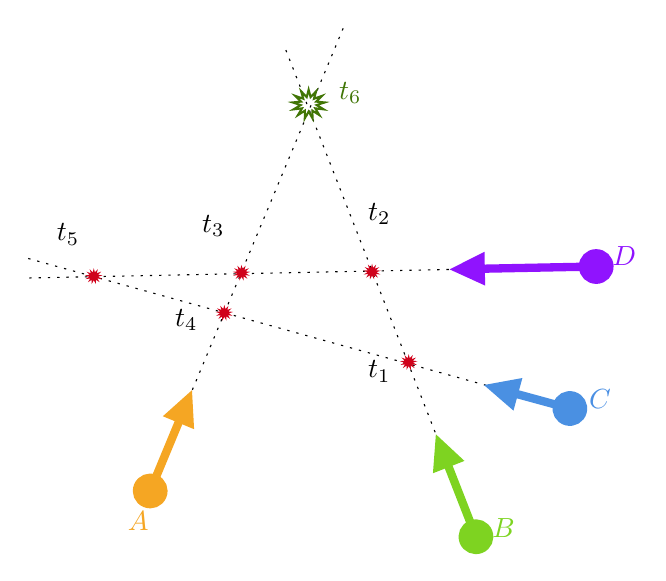
\begin{tikzpicture}[x=0.75pt,y=0.75pt,yscale=-1,xscale=1]
%uncomment if require: \path (0,11143); %set diagram left start at 0, and has height of 11143

%Straight Lines [id:da4257880873279283] 
\draw  [dash pattern={on 0.84pt off 2.51pt}]  (251.22,4004.97) -- (158.26,4227.86) ;
\draw [shift={(158.26,4227.86)}, rotate = 112.64] [color={rgb, 255:red, 0; green, 0; blue, 0 }  ][fill={rgb, 255:red, 0; green, 0; blue, 0 }  ][line width=0.75]      (0, 0) circle [x radius= 3.35, y radius= 3.35]   ;
%Straight Lines [id:da9952714607108861] 
\draw  [dash pattern={on 0.84pt off 2.51pt}]  (223.63,4015.45) -- (315.21,4249.92) ;
\draw [shift={(315.21,4249.92)}, rotate = 68.66] [color={rgb, 255:red, 0; green, 0; blue, 0 }  ][fill={rgb, 255:red, 0; green, 0; blue, 0 }  ][line width=0.75]      (0, 0) circle [x radius= 3.35, y radius= 3.35]   ;
%Straight Lines [id:da9393707554836688] 
\draw  [dash pattern={on 0.84pt off 2.51pt}]  (99.5,4115.86) -- (360.45,4188.13) ;
\draw [shift={(360.45,4188.13)}, rotate = 15.48] [color={rgb, 255:red, 0; green, 0; blue, 0 }  ][fill={rgb, 255:red, 0; green, 0; blue, 0 }  ][line width=0.75]      (0, 0) circle [x radius= 3.35, y radius= 3.35]   ;
%Straight Lines [id:da4242707810533324] 
\draw  [dash pattern={on 0.84pt off 2.51pt}]  (100.05,4125.24) -- (373.14,4119.72) ;
\draw [shift={(373.14,4119.72)}, rotate = 358.84] [color={rgb, 255:red, 0; green, 0; blue, 0 }  ][fill={rgb, 255:red, 0; green, 0; blue, 0 }  ][line width=0.75]      (0, 0) circle [x radius= 3.35, y radius= 3.35]   ;
%Straight Lines [id:da5822274503273119] 
\draw [color={rgb, 255:red, 126; green, 211; blue, 33 }  ,draw opacity=1 ][line width=3]    (315.21,4249.92) -- (298.09,4206.13) ;
\draw [shift={(295.9,4200.55)}, rotate = 68.64] [fill={rgb, 255:red, 126; green, 211; blue, 33 }  ,fill opacity=1 ][line width=0.08]  [draw opacity=0] (16.97,-8.15) -- (0,0) -- (16.97,8.15) -- cycle    ;
\draw [shift={(315.21,4249.92)}, rotate = 248.64] [color={rgb, 255:red, 126; green, 211; blue, 33 }  ,draw opacity=1 ][fill={rgb, 255:red, 126; green, 211; blue, 33 }  ,fill opacity=1 ][line width=3]      (0, 0) circle [x radius= 6.37, y radius= 6.37]   ;
%Straight Lines [id:da051074197187332526] 
\draw [color={rgb, 255:red, 245; green, 166; blue, 35 }  ,draw opacity=1 ][line width=3]    (158.26,4227.86) -- (176.09,4184.85) ;
\draw [shift={(178.39,4179.31)}, rotate = 112.53] [fill={rgb, 255:red, 245; green, 166; blue, 35 }  ,fill opacity=1 ][line width=0.08]  [draw opacity=0] (16.97,-8.15) -- (0,0) -- (16.97,8.15) -- cycle    ;
\draw [shift={(158.26,4227.86)}, rotate = 292.53] [color={rgb, 255:red, 245; green, 166; blue, 35 }  ,draw opacity=1 ][fill={rgb, 255:red, 245; green, 166; blue, 35 }  ,fill opacity=1 ][line width=3]      (0, 0) circle [x radius= 6.37, y radius= 6.37]   ;
%Straight Lines [id:da17569860173881802] 
\draw [color={rgb, 255:red, 74; green, 144; blue, 226 }  ,draw opacity=1 ][line width=3]    (360.45,4188.13) -- (324.86,4178.41) ;
\draw [shift={(319.07,4176.82)}, rotate = 15.29] [fill={rgb, 255:red, 74; green, 144; blue, 226 }  ,fill opacity=1 ][line width=0.08]  [draw opacity=0] (16.97,-8.15) -- (0,0) -- (16.97,8.15) -- cycle    ;
\draw [shift={(360.45,4188.13)}, rotate = 195.29] [color={rgb, 255:red, 74; green, 144; blue, 226 }  ,draw opacity=1 ][fill={rgb, 255:red, 74; green, 144; blue, 226 }  ,fill opacity=1 ][line width=3]      (0, 0) circle [x radius= 6.37, y radius= 6.37]   ;
%Straight Lines [id:da02986144608238317] 
\draw [color={rgb, 255:red, 144; green, 19; blue, 254 }  ,draw opacity=1 ][line width=3]    (373.14,4119.72) -- (308.52,4120.98) ;
\draw [shift={(302.52,4121.1)}, rotate = 358.88] [fill={rgb, 255:red, 144; green, 19; blue, 254 }  ,fill opacity=1 ][line width=0.08]  [draw opacity=0] (16.97,-8.15) -- (0,0) -- (16.97,8.15) -- cycle    ;
\draw [shift={(373.14,4119.72)}, rotate = 178.88] [color={rgb, 255:red, 144; green, 19; blue, 254 }  ,draw opacity=1 ][fill={rgb, 255:red, 144; green, 19; blue, 254 }  ,fill opacity=1 ][line width=3]      (0, 0) circle [x radius= 6.37, y radius= 6.37]   ;
%Shape: Star [id:dp4652455317009081] 
\draw  [draw opacity=0][fill={rgb, 255:red, 208; green, 2; blue, 27 }  ,fill opacity=1 ] (202.25,4118.9) -- (202.76,4120.88) -- (204.24,4119.34) -- (203.67,4121.31) -- (205.77,4120.56) -- (204.25,4122.07) -- (206.5,4122.29) -- (204.38,4122.99) -- (206.25,4124.13) -- (204.01,4123.85) -- (205.09,4125.65) -- (203.25,4124.47) -- (203.28,4126.51) -- (202.25,4124.69) -- (201.23,4126.51) -- (201.26,4124.47) -- (199.42,4125.65) -- (200.49,4123.85) -- (198.26,4124.13) -- (200.13,4122.99) -- (198.01,4122.29) -- (200.25,4122.07) -- (198.73,4120.56) -- (200.84,4121.31) -- (200.27,4119.34) -- (201.74,4120.88) -- cycle ;
%Shape: Star [id:dp17943360623521842] 
\draw  [draw opacity=0][fill={rgb, 255:red, 208; green, 2; blue, 27 }  ,fill opacity=1 ] (131.08,4120.55) -- (131.6,4122.54) -- (133.07,4120.99) -- (132.5,4122.97) -- (134.6,4122.22) -- (133.08,4123.73) -- (135.33,4123.95) -- (133.21,4124.64) -- (135.08,4125.78) -- (132.84,4125.51) -- (133.92,4127.3) -- (132.08,4126.12) -- (132.11,4128.16) -- (131.08,4126.34) -- (130.06,4128.16) -- (130.09,4126.12) -- (128.25,4127.3) -- (129.33,4125.51) -- (127.09,4125.78) -- (128.96,4124.64) -- (126.84,4123.95) -- (129.09,4123.73) -- (127.57,4122.22) -- (129.67,4122.97) -- (129.1,4120.99) -- (130.57,4122.54) -- cycle ;
%Shape: Star [id:dp03789410132743454] 
\draw  [draw opacity=0][fill={rgb, 255:red, 208; green, 2; blue, 27 }  ,fill opacity=1 ] (265.15,4118.34) -- (265.66,4120.33) -- (267.13,4118.79) -- (266.56,4120.76) -- (268.67,4120.01) -- (267.15,4121.52) -- (269.39,4121.74) -- (267.27,4122.44) -- (269.14,4123.57) -- (266.91,4123.3) -- (267.98,4125.1) -- (266.14,4123.92) -- (266.17,4125.96) -- (265.15,4124.14) -- (264.12,4125.96) -- (264.15,4123.92) -- (262.31,4125.1) -- (263.39,4123.3) -- (261.15,4123.57) -- (263.02,4122.44) -- (260.9,4121.74) -- (263.15,4121.52) -- (261.63,4120.01) -- (263.73,4120.76) -- (263.16,4118.79) -- (264.64,4120.33) -- cycle ;
%Shape: Star [id:dp6092374284959783] 
\draw  [draw opacity=0][fill={rgb, 255:red, 208; green, 2; blue, 27 }  ,fill opacity=1 ] (193.98,4138.2) -- (194.49,4140.19) -- (195.96,4138.65) -- (195.4,4140.62) -- (197.5,4139.87) -- (195.98,4141.38) -- (198.22,4141.6) -- (196.1,4142.3) -- (197.98,4143.44) -- (195.74,4143.16) -- (196.81,4144.96) -- (194.97,4143.78) -- (195,4145.82) -- (193.98,4144) -- (192.95,4145.82) -- (192.98,4143.78) -- (191.14,4144.96) -- (192.22,4143.16) -- (189.98,4143.44) -- (191.86,4142.3) -- (189.73,4141.6) -- (191.98,4141.38) -- (190.46,4139.87) -- (192.56,4140.62) -- (191.99,4138.65) -- (193.47,4140.19) -- cycle ;
%Shape: Star [id:dp9525934681135235] 
\draw  [draw opacity=0][fill={rgb, 255:red, 208; green, 2; blue, 27 }  ,fill opacity=1 ] (282.8,4161.93) -- (283.31,4163.91) -- (284.79,4162.37) -- (284.22,4164.34) -- (286.32,4163.6) -- (284.8,4165.1) -- (287.05,4165.32) -- (284.92,4166.02) -- (286.8,4167.16) -- (284.56,4166.89) -- (285.64,4168.68) -- (283.79,4167.5) -- (283.82,4169.54) -- (282.8,4167.72) -- (281.78,4169.54) -- (281.81,4167.5) -- (279.97,4168.68) -- (281.04,4166.89) -- (278.8,4167.16) -- (280.68,4166.02) -- (278.56,4165.32) -- (280.8,4165.1) -- (279.28,4163.6) -- (281.38,4164.34) -- (280.81,4162.37) -- (282.29,4163.91) -- cycle ;
%Shape: Star [id:dp7689921001871347] 
\draw  [color={rgb, 255:red, 65; green, 117; blue, 5 }  ,draw opacity=1 ][line width=0.75]  (234.6,4034.49) -- (235.53,4038.11) -- (238.22,4035.29) -- (237.18,4038.89) -- (241.01,4037.52) -- (238.24,4040.27) -- (242.33,4040.67) -- (238.47,4041.94) -- (241.88,4044.01) -- (237.81,4043.52) -- (239.77,4046.78) -- (236.41,4044.63) -- (236.47,4048.35) -- (234.6,4045.04) -- (232.74,4048.35) -- (232.79,4044.63) -- (229.44,4046.78) -- (231.4,4043.52) -- (227.32,4044.01) -- (230.74,4041.94) -- (226.87,4040.67) -- (230.96,4040.27) -- (228.19,4037.52) -- (232.02,4038.89) -- (230.98,4035.29) -- (233.67,4038.11) -- cycle ;

% Text Node
\draw (146.27,4236.75) node [anchor=north west][inner sep=0.75pt]   [align=left] {$\displaystyle \textcolor[rgb]{0.96,0.65,0.14}{A}$};
% Text Node
\draw (321.83,4240.13) node [anchor=north west][inner sep=0.75pt]   [align=left] {$\displaystyle \textcolor[rgb]{0.49,0.83,0.13}{B}$};
% Text Node
\draw (368.42,4177.79) node [anchor=north west][inner sep=0.75pt]   [align=left] {$\displaystyle \textcolor[rgb]{0.29,0.56,0.89}{C}$};
% Text Node
\draw (379.64,4108.83) node [anchor=north west][inner sep=0.75pt]   [align=left] {$\displaystyle \textcolor[rgb]{0.56,0.07,1}{D}$};
% Text Node
\draw (262,4164) node [anchor=north west][inner sep=0.75pt]   [align=left] {$\displaystyle t_{1}$};
% Text Node
\draw (262,4088) node [anchor=north west][inner sep=0.75pt]   [align=left] {$\displaystyle t_{2}$};
% Text Node
\draw (182,4094) node [anchor=north west][inner sep=0.75pt]   [align=left] {$\displaystyle t_{3}$};
% Text Node
\draw (169,4139) node [anchor=north west][inner sep=0.75pt]   [align=left] {$\displaystyle t_{4}$};
% Text Node
\draw (112,4098) node [anchor=north west][inner sep=0.75pt]   [align=left] {$\displaystyle t_{5}$};
% Text Node
\draw (248,4030) node [anchor=north west][inner sep=0.75pt]   [align=left] {$\displaystyle \textcolor[rgb]{0.25,0.46,0.02}{t_{6}}$};


\end{tikzpicture}
    }
\end{center}
Với $5$ cặp gặp nhau, ta có điều kiện gặp của $5$ cặp điểm này là:
\begin{align*}
\left\{
    \begin{array}{rrrr}
    \left(\Vec{r_B} - \Vec{r_C} \right)   & = & t_1 \left( \Vec{v_B} - \Vec{v_C} \right) & \text{(cặp B-C).} \\
    \left(\Vec{r_B} - \Vec{r_D} \right)   & = & t_2 \left( \Vec{v_B} - \Vec{v_D} \right) & \text{(cặp B-D).} \\
    \left(\Vec{r_A} - \Vec{r_D} \right)   & = & t_3 \left( \Vec{v_A} - \Vec{v_D} \right) & \text{(cặp A-D).} \\
    \left(\Vec{r_C} - \Vec{r_A} \right)   & = & t_4 \left( \Vec{v_C} - \Vec{v_A} \right) & \text{(cặp C-A).} \\
    \left(\Vec{r_C} - \Vec{r_D} \right)   & = & t_5 \left( \Vec{v_C} - \Vec{v_D} \right) & \text{(cặp D-C).} \\
    \end{array}
\right.
\end{align*}
Từ hệ phương trình trên, ta khử $\Vec{r_C}, \Vec{r_D}, \Vec{v_C}, \Vec{v_D}$ ta sẽ thu được phương trình sau:
\begin{align}
    \Vec{r_A} - \Vec{r_B} & =  \frac{t_1 t_2 \left(t_4 - t_3 \right) + t_2 t_4 \left( t_3 - t_5 \right) +t_1 t_3 \left(t_5 - t_4 \right)}{t_5 \left( t_1 + t_3 - t_2 - t_4 \right) - t_1 t_3 - t_2 t_4} \left( \Vec{v_A} - \Vec{v_B} \right) = t_6 \left( \Vec{v_A} - \Vec{v_B} \right).
    \label{S2_eq.1.1}
\end{align}
Như vậy từ biểu thức (\ref{S2_eq.1.1}) ta thấy rằng cặp điểm $\left(A-B\right)$ có va chạm nhau. Như vậy có $6$ va chạm diễn ra.
\item 
\begin{figure}[ht]
    \centering
    \includegraphics[scale=0.45]{Problem_1/Image/S2.2.1.png}
    \caption{}
    \label{S2.2.1}
\end{figure}

Ta sẽ biến một hệ 2D thành một hệ 1D bằng hình (\ref{S2.2.1}). Một số điểm cần lưu ý:
\begin{enumerate}
    \item Do các bạn đều va chạm mỗi khi đi va điểm giao nhau của 2 quỹ đạo. Nên khi hình ảnh hai bạn trùng nhau trên màn tương đương hai bạn va chạm.
    \item Hành động va chạm vẫn tuân theo quy tắc mà đề bài đã đề ra là trao đổi tốc độ và quỹ đạo.
\end{enumerate}
{ \textbf{Tổng va chạm diễn ra}}

Hình (\ref{S2.2.2}) mô tả hai trường hợp. Nếu \textit{không phân biệt} rõ hạt $C'$ hay hạt $D'$ thì giống như hai hạt \textit{đi xuyên qua nhau mà không tương tác gì}. 
\begin{figure}[ht]
    \centering
    \includegraphics[scale=0.45]{Problem_1/Image/S2.2.2.png}
    \caption{}
    \label{S2.2.2}
\end{figure}
\\
Vậy lúc này nếu nói về số va chạm tổng cộng thì phần 2 vẫn có hiện tượng giống như phần 1. Như vậy tổng số va chạm diễn ra vẫn là \textbf{6}.

\textit{Đến đây ta vô tình bổ sung thêm cho nhận định 1 trong phần lưu ý.}

{ \textbf{Phân loại loại hạt trên màn.}}
\\Từ giờ để dễ gọi, ta sẽ thay thế từ `\textit{bạn}' thành `\textit{hạt}'. 

Lúc này thì bài toán đã trở thành một bài toán va chạm 1D. Các vận tốc của các hạt là bất kì, nhưng vẫn thoả mãn điều kiện ở Phần 1.
\begin{figure}[ht]
    \centering
    \includegraphics[scale=0.6]{Problem_1/Image/S2.2.3.png}
    \caption{}
    \label{S2.2.3}
\end{figure}
\\
Từ đây ta chia các hạt trên màn gồm: \textbf{hạt ngoài rìa} ($A'$ và $D'$) và \textbf{hạt bên trong} ($B'$ và $C'$).

Lý do để chia cũng khá dễ hiểu, ta thấy rằng tiềm năng để hạt ngoài rìa va chạm ít hơn so với lại hạt bên trong. Hạt ngoài rìa tự do một đầu, nên khả năng thoát khỏi hệ sớm hơn hạt bên trong. Giờ ta sẽ đi khảo sát số va chạm của các loại hạt này.

\textbf{Hạt ngoài rìa:}

Để số va chạm có thể được tối đa thì

\textit{Điều kiện 1}: Tất các hạt phải \textit{hướng vận tốc về phía hạt $D'$}. Lý do là vì để cho hạt $D'$ có khả năng trao đổi vận tốc với hạt đó. Vì vậy số va chạm lớn nhất của $D'$ diễn ra khi các hạt đều hướng về phía $D'$.
\begin{figure}[ht]
    \centering
    \includegraphics[scale=0.6]{Problem_1/Image/S2.2.4.png}
    \caption{}
    \label{S2.2.4}
\end{figure}

\textit{Điều kiện 2:} Hạt $D'$ phải va chạm với những hạt có tốc độ thấp và lần lượt đến các hạt có tốc độ cao sau. Bởi vì nếu hạt $C'$ đuổi theo hạt $D'$, mà tốc độ của $C'$ nhỏ hơn của $D'$ thì hạt $D'$ sẽ thoát khỏi hệ và kết thúc quá trình va chạm. Vì thế mình chia các loại tốc độ thành: \textit{Lớn-Trung-Nhỏ}

\begin{center}
\begin{tabular}{|l|c|}
\hline
Thứ tự va chạm    & Số va chạm của $D'$ \\ \hline
Lớn               & 1                   \\ \hline
Trung(Nhỏ) - Lớn  & 2                   \\ \hline
Nhỏ - Trung - Lớn & 3                   \\ \hline
\end{tabular}
\end{center}


Nhìn vào bảng thì ta thấy số va chạm khả dĩ của hạt ngoài rìa là \textbf{[1;3]}.

\textbf{Hạt bên trong:}
\\
Ta sẽ lấy đại diện là hạt $B'$. Dựa vào kết quả đã được tính ở những hạt ngoài rìa, ta lập luận được số va chạm mà \textit{không có sự góp mặt của $D'$} là \textbf{[3;5]}. Lý do là bởi tổng số va chạm vẫn bảo toàn là \textbf{6}.

Các hạt $A'$ và $C'$ không thể va chạm trực tiếp với nhau. Lý do là vì khi $C'$ gặp $B'$ thì đã bị bật ra do va chạm đàn hồi. Tương tự với $A'$. Vì thế nên sẽ không có va chạm giữa $A'$ và $C'$, số va chạm là $0$.


\begin{figure}[ht]
    \centering
    \includegraphics[scale=0.6]{Problem_1/Image/S2.2.5.png}
    \caption{Tương tác của $A'-B'-C'$}
    \label{S2.2.5}
\end{figure}

Do số va chạm của các hạt còn lại (là $A'$, $B'$, $C'$) gồm va chạm giữa $B'-C'$, $B'-A'$ (cặp $A'-C'$ không thể xảy ra va chạm như vừa chứng minh). Chung quy đều là va chạm có mặt $B'$. Như vậy số va chạm mà $B'$ trải nghiệm thuộc \textbf{[3;5]}.

 \textbf{Tổng kết}
\\
\begin{center}
    \begin{tabular}{|l|c|}
\hline
              & Số va chạm khả dĩ                   \\ \hline
Hạt ngoài rìa & \textbf{[1;3]} \\ \hline
Hạt bên trong & \textbf{[3;5]} \\ \hline
\end{tabular}
\end{center}
Từ đây dễ dàng kết luận là số va chạm lớn nhất một hạt (bạn) có thể trải nghiệm là \textbf{5}.
\item \textbf{Phổ điểm}

\begin{center}

\begin{tabular}{|c|p{3.5cm}|p{7.5cm}|c|}
\hline
\multicolumn{1}{|l|}{Phần} &
  \multicolumn{2}{l|}{Nội dung} &
  \multicolumn{1}{l|}{Điểm thành phần} \\ \hline
\multirow{6}{*}{1} &
  \multicolumn{1}{l|}{\multirow{3}{*}{Nếu làm theo cách 1}} &
  Biểu diễn chuyển động trên trục Oxyt. &
  0.5 \\ \cline{3-4} 
                   & \multicolumn{1}{l|}{} & Biện luận 3 đồ thị bất kì đồng phẳng.         & 1    \\ \cline{3-4} 
 &
  \multicolumn{1}{l|}{} &
  Kết luận 4 đồ thị đồng phẳng, suy ra có cuộc gặp nhau thứ 6. &
  0.5 \\ \cline{2-4} 
 &
  \multicolumn{1}{l|}{\multirow{3}{*}{Nếu làm theo cách 2}} &
  Biện luận chuyển động trong hệ quy chiếu gắn với một người. &
  0.5 \\ \cline{3-4} 
                   & \multicolumn{1}{l|}{} & Biện luận các đường thẳng quỹ đạo trùng nhau. & 1    \\ \cline{3-4} 
                   & \multicolumn{1}{l|}{} & Kết luận cuộc gặp nhau thứ 6 có xảy ra.       & 0.5  \\ \hline
\multirow{7}{*}{2} & \multicolumn{2}{l|}{Tương đương hệ 2D và 1D.}                                            & 0.5 \\ \cline{2-4} 
                   & \multicolumn{2}{l|}{Chứng minh tổng số va chạm.}                      & 0.25 \\ \cline{2-4} 
                   & \multicolumn{2}{l|}{Điều kiện 1: Hạt ngoài rìa.}                      & 0.25  \\ \cline{2-4} 
                   & \multicolumn{2}{l|}{Điều kiện 2: Hạt ngoài rìa.}                      & 0.25 \\ \cline{2-4} 
                   & \multicolumn{2}{l|}{Va chạm khả dĩ hạt ngoài rìa.}                    & 0.25 \\ \cline{2-4} 
                   & \multicolumn{2}{l|}{Chứng minh cặp hạt A-C không va chạm.}            & 0.25 \\ \cline{2-4} 
                   & \multicolumn{2}{l|}{Va chạm khả dĩ hạt bên trong.}                    & 0.25 \\ \hline
\end{tabular}

\end{center}
Nếu làm theo cách khác nhưng hợp lý thì được trọn điểm.
\end{enumerate}